\chapter{REGALE}
REGALE\cite{REGALE} è un progetto open source nato ad Aprile 2021 che ha come compito quello di costruire uno stack software scalabile per migliorare l'efficenza di sistemi Exascale\footnote{Exascale: capace di eseguire operazioni nell'ordine di ExaFlops ($10^{18}$)} HPC. Questo progetto è particolarmente interessante nell'ambito del Power Management in quanto si è proposta di implementare la quasi totalità degli attori proposti nello dello stato dell'arte per quanto riguarda il Power Management di sistemi di HPC.
\section{Obbiettivi}

\section{Power Stack}
Molti dei componenti mostrati nel modello del Power Stack \ref{fig:powerstackscheme} sono stati sviluppati e resi disponibili nel progetto di REGALE. A questi mancano solo il \emph{Workflow engine} ed un \emph{Resource manager} specifico.
\begin{figure}[H]
    \centering
    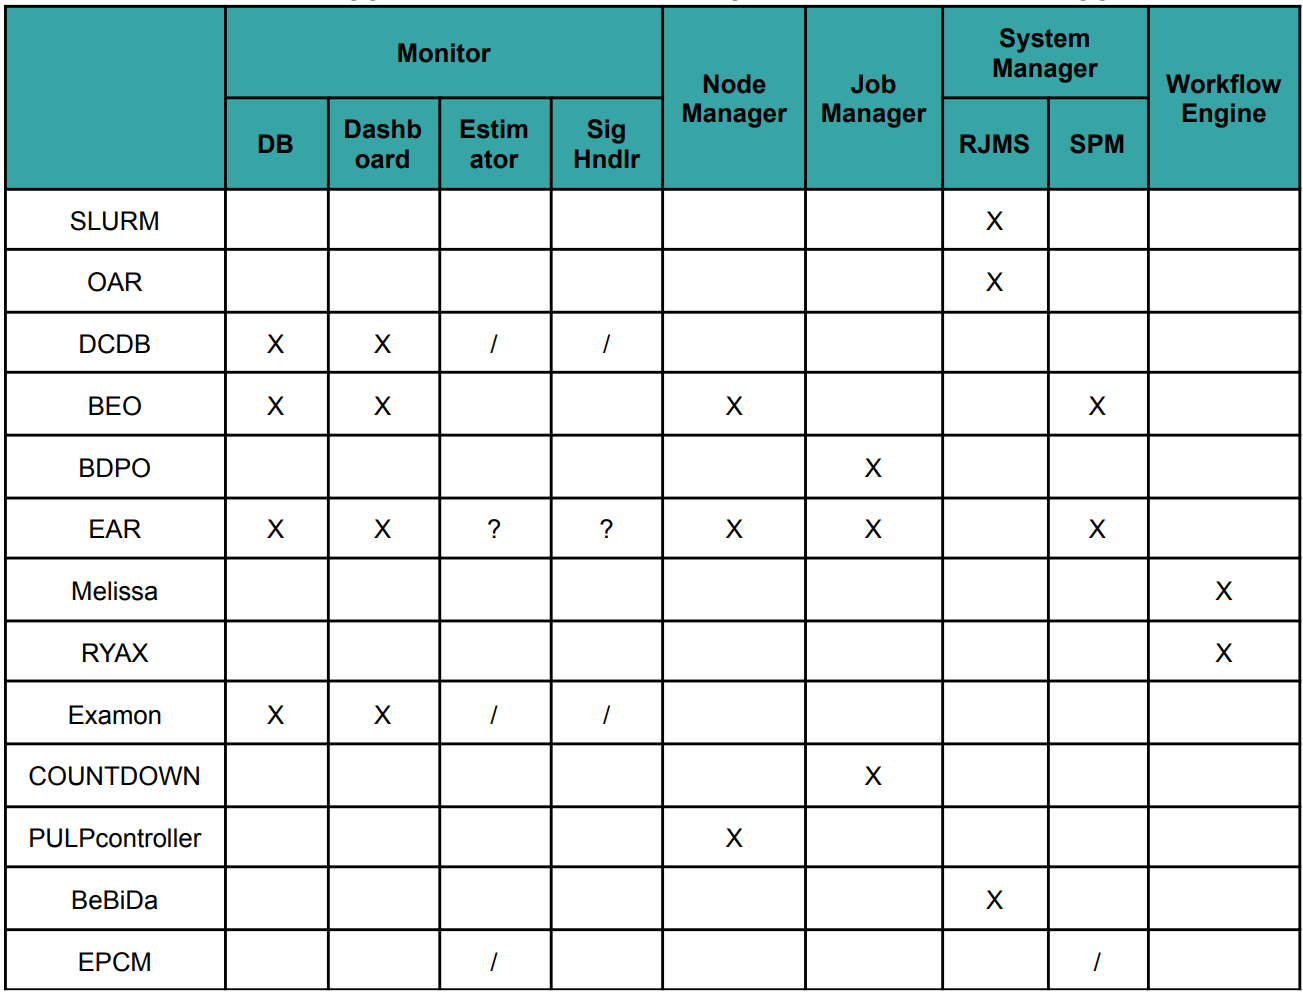
\includegraphics[width=\textwidth]{./img/REGALE-components.png}
    \caption{Copertura componenti REGALE}
    \label{fig:regale_cover}
\end{figure}
\section{Problematica}
Vista l'implementazione proposta, il problema con il quale si sta interfacciando il progetto può essere descritto con mancanza di interoperabilità. Ciò che manca in REGALE, è un layer di comunicazione che permetta ai vari attori di comunicare tra di loro. Infatti sono stati prima proposti diversi modelli di interazione tra i vari componenti a due a due, fino a quando si è deciso di provare a sviluppare un ulteriore middleware che standardizzasse le comunicazioni tra i vari attori, utilizzando un singolo strumento per tutti i componenti. 
%Il problema è che non sono interoperabili